% Author :  Lionel du Peloux
% Contact : lionel.dupeloux@gmail
% Year : 2017

% ===========================
% COMPILER DIRECTIVES
% ===========================
% !TEX encoding = UTF-8 Unicode
% !TEX TS-program = XeLaTeX-shellescape
% !BIB TS-program = biber
% !BIB program = biber

\PassOptionsToPackage{cover}{blurb}

% ACTIVATE TO TRIM BLEED MARGINS
% \PassOptionsToPackage{nobleed}{blurb}

% SELECT COVER TYPE
% \PassOptionsToPackage{hardcover}{blurb}
\PassOptionsToPackage{softcover}{blurb}

% DEBUG OPTIONS
\PassOptionsToPackage{showbleed}{blurb}
\PassOptionsToPackage{showspine}{blurb}
\PassOptionsToPackage{showisbn}{blurb}
% \PassOptionsToPackage{showrules}{blurb}


\documentclass[12pt,fleqn]{thesis}
	\graphicspath{{./ch7_numeric/img/}{./ch6_kirchhoff/img/}{./ch5_energy/img/}{./ch4_geometry/img/}{./ch3_creteil/img/}{./ch2_gridshell/img/}{./cover/}}
	\addbibresource{library.bib}

\newlength\CoverWidth
\newlength\MainBarYOffset
\newlength\MainBarHeight
\newlength\MainBarStepWidth
\newlength\MainTextXMargin
\newlength\AuthorYMargin
\newlength\AuthorWidth
\newlength\AuthorRuleWidth
\newlength\BackTitleTopMargin
\newlength\BackTitleSideMargin
\newlength\BackTextYOffset
\newlength\BackTickMargin
%
\setlength{\CoverWidth}{\PaperWidth/2-\BleedOuterMargin-\BlurbGutterWidth/2}
%
\setlength{\MainBarYOffset}{\PageHeight/2}
\setlength{\MainBarHeight}{2.5cm}
\setlength{\MainBarStepWidth}{2cm}
\setlength{\MainTextXMargin}{2cm}
%
\setlength{\AuthorYMargin}{1.5cm}
\setlength{\AuthorRuleWidth}{4mm}
%
\setlength{\BackTitleTopMargin}{3cm}
\setlength{\BackTitleSideMargin}{3.0cm}
\setlength{\BackTickMargin}{0.5cm}

% FONT FAMILY
\newfontfamily\FTRegular{FuturaLT}[Scale = MatchUppercase]
\newfontfamily\FTLight{FuturaLT-Light}[Scale = MatchUppercase]
\newfontfamily\FTBold{FuturaLT-Bold}[Scale = MatchUppercase]
\newfontfamily\FTHeavy{FuturaLT-Heavy}[Scale = MatchUppercase]
\newfontfamily\FTBookOblique{FuturaLT-BookOblique}[Scale = MatchUppercase]
\newfontfamily\FTCondensedBoldOblique{FuturaLT-CondensedBoldOblique}[Scale = MatchUppercase]
\newfontfamily\GSLight{GillSans-Light}[Scale = MatchUppercase]
\newfontfamily\FTCondensed{FuturaLT-Condensed}[Scale = MatchUppercase]

% TYPE FACE FRONT COVER
\DeclareRobustCommand{\tfgridshell}{\FTBold\fontsize{70pt}{0pt}\selectfont}
\DeclareRobustCommand{\tfelastica}{\FTLight\fontsize{60pt}{0pt}\selectfont}
\DeclareRobustCommand{\tfauthor}{\FTRegular\fontsize{16pt}{0pt}\selectfont}
\DeclareRobustCommand{\tfyear}{\FTHeavy\fontsize{25pt}{0pt}\selectfont}
\DeclareRobustCommand{\tfphd}{\FTHeavy\fontsize{30pt}{0pt}\selectfont}
% TYPE FACE BACK COVER
\DeclareRobustCommand{\tfHA}{\FTBookOblique\fontsize{15pt}{0pt}\selectfont}
\DeclareRobustCommand{\tfHB}{\FTBold\fontsize{16pt}{0pt}\selectfont}
\DeclareRobustCommand{\tfquote}{\FTCondensedBoldOblique\large}
\DeclareRobustCommand{\tftxt}{\GSLight\small}
% TYPE FACE SPINE
\DeclareRobustCommand{\tfspineauthor}{\FTRegular\fontsize{22pt}{0pt}\selectfont}
\DeclareRobustCommand{\tfspinephd}{\FTCondensed\fontsize{14pt}{0pt}\selectfont}
\DeclareRobustCommand{\tfspinetitle}{\FTBold\fontsize{36pt}{0pt}\selectfont\color{secondary}}

\let\defaultpgflinewidth\pgflinewidth
\setlength{\pgflinewidth}{0pt}

\usepackage{multicol}
\usepackage{adjustbox}
\usepackage{soul}
\usepackage{wrapfig}

% no addvspace
\makeatletter
\patchcmd{\mult@@cols}
	{\addvspace\multicolsep}
	{}
	{}{}
\patchcmd{\endmulticols}
	{\addvspace\multicolsep}
	{}
	{}{}
\makeatother

\begin{document}
\thispagestyle{empty}
\AddToShipoutPictureBG*{%
	% BACK COVER
	\begin{tikzpicture}[remember picture, overlay, inner sep=0pt]
		% background color
		\definecolor{graybckgd}{gray}{0.9}
		\path[fill,graybckgd] (PPbl) rectangle (PPtr);
		% main bar nodes
		\path (PGtl -| PPtr) node[yshift=-\MainBarYOffset] (MBtr) {};
		\path (MBtr -| SPtl) node[xshift=-\MainBarStepWidth, yshift=-\MainBarHeight] (MBbl) {};
		\coordinate[yshift=\MainBarHeight] (MBtl) at (MBbl);
		\coordinate[yshift=-\MainBarHeight] (MBbr) at (MBtr);
		% image mask
		\begin{scope}
			\clip (SPtr |- MBtr) rectangle (PPtr);
			\node[anchor=north east, xshift=0cm, yshift=0cm] at (PPtr)
				{\adjustbox{}{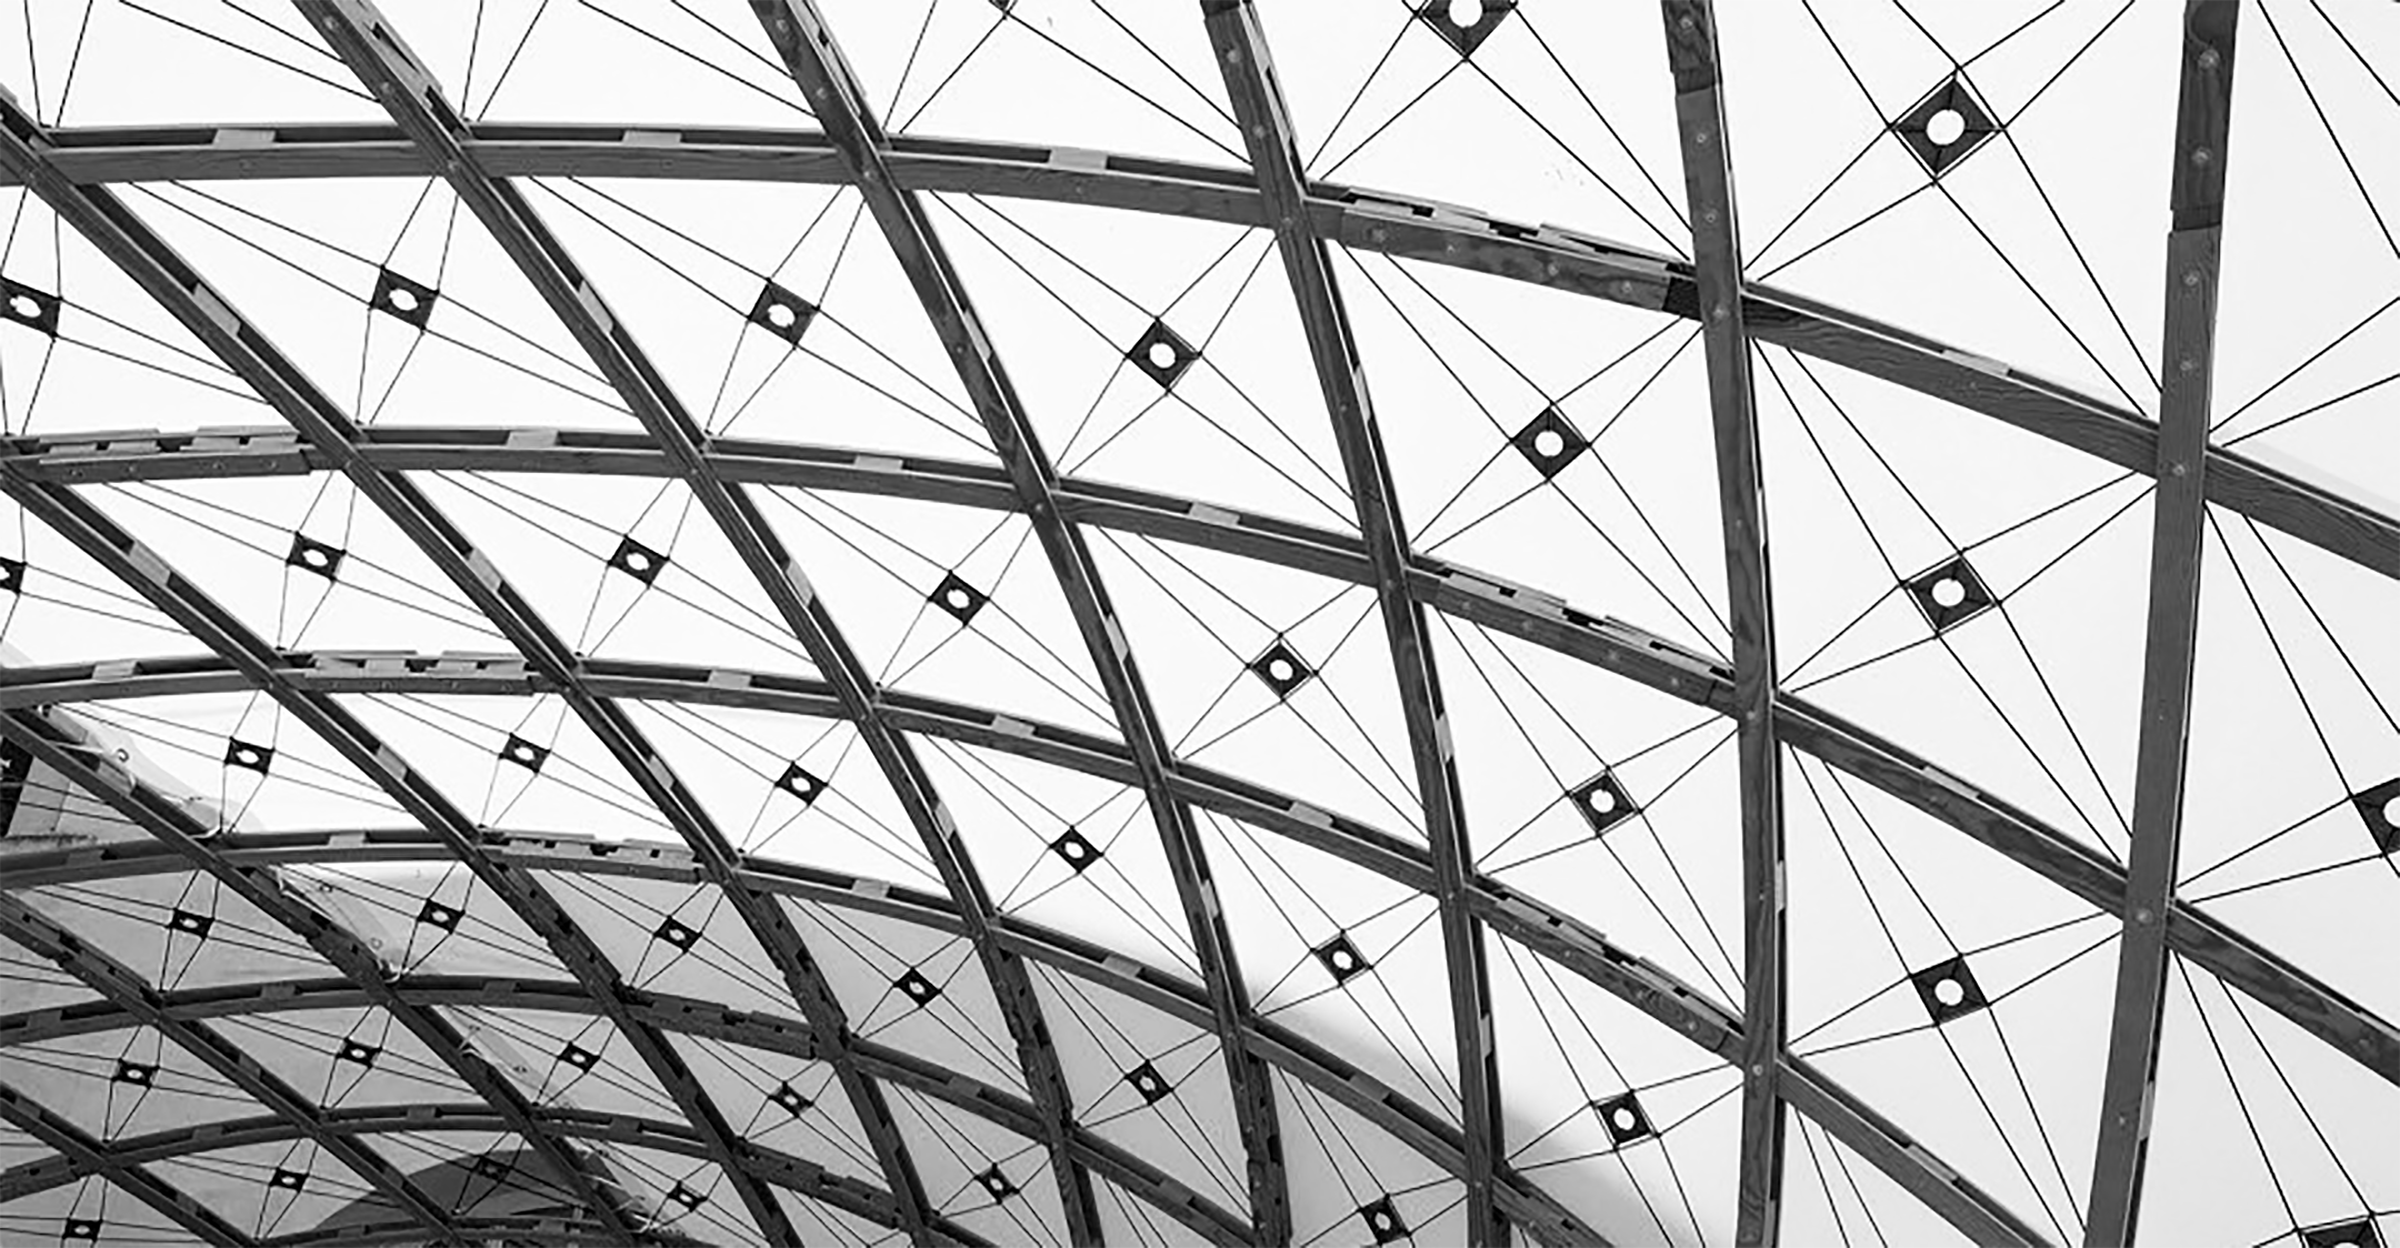
\includegraphics[width=30cm]{fav_nb.png}}};
		\end{scope}		
		% main bar
		\path[fill,black,opacity=1]  (MBbl) rectangle (MBtr -| PPtr);
		\node[anchor=east, xshift=-\MainTextXMargin, yshift=\MainBarHeight/2] at (MBbr){%
			\fbox{\parbox[b]{16cm}{\raggedleft\color{white}\tfelastica ELASTIC}}};
		\node[anchor=east, xshift=-\MainTextXMargin, yshift=-\MainBarHeight/2] at (MBbr){%
			\fbox{\parbox[b]{16cm}{\raggedleft\color{secondary}\tfgridshell GRIDSHELL}}};
	\end{tikzpicture}
	%
	\begin{tikzpicture}[remember picture, inner sep=0pt]
		% author bar
		\node[anchor=south east, xshift=-\MainTextXMargin, yshift=\AuthorYMargin] at (PGbr -| PPtr){%
			\fbox{\hbox{\tfauthor Lionel du Peloux}}};
		\coordinate (AHbl) at (current bounding box.south west);
		\coordinate (AHbr) at (current bounding box.south east);
		\coordinate (AHtl) at (current bounding box.north west);
		\coordinate (AHtr) at (current bounding box.north east);
		\path[fill,black] ([yshift=-2mm]AHbl) rectangle ([yshift=-4mm]AHbr);
		% year
		\node[anchor=center, yshift=\MainBarHeight/2] (MByear) at (MBbr -| PPt){%
			\fbox{\hbox{\color{white}\tfyear 2017}}};
		% phd
		\node[anchor=center, xshift=-\MainBarStepWidth/2, rotate=90] (MBphd) at (MByear -| SPtl){%
			\fbox{\hbox{\color{white}\tfphd PhD}}};
		\path (PGb) -- (PGb |- MBbr) coordinate[midway] (Pt);
		\pgfresetboundingbox
		\path[use as bounding box] (0,0);
	\end{tikzpicture}
	% SPINE
	\begin{tikzpicture}[remember picture, inner sep=0pt]
		% spine PHD
		\node[anchor=base, yshift=\AuthorYMargin] at (PGb){%
			\fbox{\hbox{\tfspinephd PhD Thesis}}};
		\path (current bounding box.north) -- (PGb |- MBbr) coordinate[midway] (Pt);
		\pgfresetboundingbox
		\path[use as bounding box] (0,0);
	\end{tikzpicture}
	\begin{tikzpicture}[remember picture, overlay, inner sep=0pt]
		% spine author
		\node[anchor=center, yshift=0mm, rotate=90] at (Pt){%
			\fbox{\hbox{\tfspineauthor Lionel du Peloux}}};
		% spine title
		\path (PGt) -- (PGt |- MBtr) coordinate[midway] (Pt);
		\node[anchor=center, yshift=0mm, rotate=90] at (Pt){%
			\fbox{\hbox{\tfspinetitle ELASTIC GRIDSHELL}}};
		\pgfresetboundingbox\path[use as bounding box] (0,0);
	\end{tikzpicture}
	% BACK COVER
	\sodef\spaceout{}{0pt plus 1fil}{.4em plus 1fil}{0pt}%
	\begin{tikzpicture}[remember picture, overlay, inner sep=0pt]
		\coordinate[xshift=\BackTitleSideMargin, yshift=-\BackTitleTopMargin] (HA) at (PGtl);
		\node[anchor=base west, yshift=0cm] at (HA){%
			\tfHA%
			\fbox{\parbox[b]{\CoverWidth-2\BackTitleSideMargin}{\spaceout{Modeling of bending-torsion couplings in active-bending structures}}}%
		};
		\path[fill,black] (PPtl |- HA) rectangle ([xshift=-\BackTickMargin, yshift=2mm]HA);
		\coordinate[yshift=-0.75cm] (HB) at (HA);
		\path[fill,secondary] (PPtl |- HB) rectangle ([xshift=-\BackTickMargin, yshift=4mm]HB);
		\node[anchor=base west, yshift=0cm] at (HB){%
			\tfHB%
			\fbox{\parbox[b]{\CoverWidth-2\BackTitleSideMargin}{\spaceout{APPLICATION TO THE DESIGN OF ELASTIC GRIDSHELLS}}}%
		};
		% abstract
		\setlength\columnsep{0.5cm}%
		\coordinate[yshift=-2cm] (HC) at (HB);
		\path[fill,black] (PPtl |- HC) rectangle ([xshift=-\BackTickMargin, yshift=-8mm]HC);
		\node[anchor=north west] at (HC){%
			\fbox{\parbox[t]{\CoverWidth-2\BackTitleSideMargin}{%
			\tftxt\setstretch{1.0}%
			\setlength{\parindent}{0em}%
			% cant align properly the text at the top of the box so add a small amount of negative vspace
			\vspace{-0.3\baselineskip}
			\begin{multicols}{2}%
				\noindent
				An \emph{elastic gridshell} is a freeform structure, generally doubly curved, but formed out through the reversible deformation of a regular and initially flat structural grid. Building curved shapes that may seems to offer the best of both worlds~: shell structures are amongst the most performant mechanically speaking while planar and orthogonal constructions are much more efficient and economic to produce than curved ones. This ability to \textquote{form a form} efficiently is of peculiar importance in the current context where morphology is a predominant component of modern architecture, and envelopes appear to be the neuralgic point for building performances.

				The concept was invented by Frei Otto, a German architect and structural engineer who devoted\vspace{7\baselineskip} many years of research to gridshells. In 1975 he designed the Multihalle of Mannheim, a 7500\,m\textsuperscript{2} wooden shell which demonstrated the feasibility of this technology and made it famous to a wide audience. However, despite their potential, very few projects of this kind were built after this major realization. And for good reason, the resources committed at that time cannot guarantee the replicability of this experiment for more standard projects, especially on the economic level. Moreover, the technics and methods developed by Otto's team in the 1960s have mostly fall into disuse or are based on disciplines that have considerably evolved. New materials, such as composite materials, have recently emerged. They go beyond the limitations of conventional materials such as timber and offer at all levels much better technical performances for this kind of application. Finally, it should be noted that the regulatory framework has also deeply changed, bringing a certain rigidity to the penetration of innovations in the building industry. Therefore, the design of gridshells arises in new terms for current architects and engineers and comes up against the inadequacy of existing tools and methods.

				In a first part, we deliver a thorough review of this topic and we present in detail one of our main achievements, the ephemeral cathedral of Créteil, built in 2013 and still in service. In a second part, \vspace{7\baselineskip}we develop an original discrete beam element with a minimal number of degrees of freedom adapted to the modeling of bending and torsion inside gridshell members with anisotropic cross-section. Enriched with a ghost node, it allows to model more accurately physical phenomena that occur at connections or at supports. Its numerical implementation is presented and validated through several test cases. Although this element has been developed specifically for the study of elastic gridshells, it can advantageously be used in any type of problem where the need for an interactive computation with elastic rods taking into account flexion-torsion couplings is required.
			\end{multicols}}}};
		\coordinate[xshift=\CoverWidth/2-\BackTitleSideMargin] (HC) at (MBphd -| HB);
		\node[anchor=center] at (HC){%
			\fbox{\parbox[c]{\CoverWidth-2\BackTitleSideMargin}{%
				\tfquote\setstretch{1.1}%
				\centering
				% \raggedleft
				In this thesis, which marks an important step in a personal research adventure initiated in 2010,\\we try to embrace the issue of the design of elastic gridshells in all its complexity,\\addressing both theoretical, technical and constructive aspects. 
			}}%
		};
	\end{tikzpicture}
}
\hbox{}
\end{document}

